\documentclass[12pt,a4paper]{article}
% \usepackage[utf8]{inputenc} % fontspecと併用時は不要
\usepackage[japanese]{babel}
\usepackage{amsmath}
\usepackage{amsfonts}
\usepackage{amssymb}
\usepackage{geometry}
\usepackage{graphicx}
\usepackage{enumitem}
\usepackage{fancyhdr}
\usepackage{verbatim}

% 日本語改行設定
\usepackage{xeCJK}
\usepackage{indentfirst}
\setlength{\parindent}{1em}

% 日本語フォント設定
\usepackage{fontspec}
\setmainfont{Hiragino Mincho Pro}
\setsansfont{Hiragino Sans}
\setmonofont{Menlo}
\setCJKmainfont{Hiragino Mincho Pro}
\setCJKsansfont{Hiragino Sans}
\setCJKmonofont{Menlo}
% ページ設定
\geometry{margin=1.5cm}
\pagestyle{fancy}
\fancyhf{}
\fancyhead[L]{プログラミング応用 第四回}
\fancyhead[R]{演習問題}
\fancyfoot[R]{\ifnum\value{page}=1\small（裏面に続く）\fi}
\fancyfoot[C]{\thepage}
\renewcommand{\headrulewidth}{0.4pt}
\renewcommand{\footrulewidth}{0.4pt}

% 問題番号のカウンター
\newcounter{problem}
\setcounter{problem}{0}

% シンプルな問題環境
\newenvironment{problem}[1][]{
    \refstepcounter{problem}
    \vspace{1em}
    \noindent
    \textbf{問\arabic{problem}} #1
    %\vspace{0.5em}
    %\par
}{
    \vspace{1em}
}

\begin{document}

% ヘッダー情報
\begin{center}
    {\Large \textbf{プログラミング応用 第四回}}\\[0.5em]
    {\large \textbf{演習問題}}\\[1em]
\end{center}

\noindent\textbf{注意事項}

\begin{itemize}[leftmargin=1em]
    \item 解答はpdf形式でLMSにアップロードしてください (例えば紙に手書きしてスキャンしたものや \TeX をコンパイルしたものなど)
    \item 締切：2025年11月4日（火）日本時間13時
    \item 質問がある場合は手を挙げてください.
    \item なお、アルゴリズムの記述問題に関しては講義資料の疑似コードを参考にしてください（明確な文法が存在するわけではないので、あくまでもアルゴリズムの動作が理解できるよう記述してあれば十分です）。記述に不安がある場合は質問すること.
    \item 講義中で説明した定理や補題は証明なしに用いてよい. また, 問題中に指定した定理や補題も証明なしに用いてよい.
\end{itemize}

\begin{problem}
次の問いに答えよ.
\begin{enumerate}
\item 次の図\ref{fig:graph_ex}で表されるグラフの隣接行列 $A$ を書け.

\begin{figure}[h]
    \begin{center}
    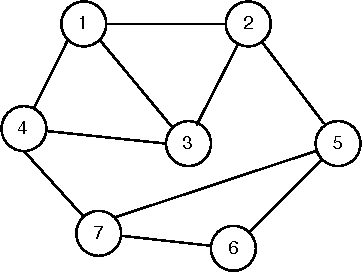
\includegraphics[width=0.45\textwidth]{graph_ex.drawio.pdf}
    \caption{グラフ \label{fig:graph_ex}}
    \end{center}
\end{figure}

\item グラフ $G=(V,E)$ の三角形の個数を $\mathrm{Tri}(G)$ とする. ここで三角形とは, 相異なる三つの頂点からなる集合 $\{u,v,w\}\subseteq V$ であって, $\{u,v\},\{v,w\},\{w,u\}\in E$ を満たすものを表す. 例えば上の図で表されるグラフの三角形は$\{1,2,3\},\{1,3,4\},\{5,6,7\}$の3つである. このとき, \[\mathrm{Tri}(G) = \frac{1}{6}\mathrm{tr}(A^3)\]を示せ. ここで$\mathrm{tr}(M)$は行列$M$のトレース (対角成分の和) を表す.

\end{enumerate}

\end{problem}

\newpage

\begin{problem}
    以下の各小問に答えよ.
    \begin{enumerate}
    \item グラフ $G=(V,E)$ の隣接行列を$A$とする. 任意の $\ell\ge 0$ と $u,v\in V$ に対して, $A^\ell_{u,v}$ は $u$ から $v$ への長さ $\ell$ の路の本数に等しいことを示せ.
    \item $n$頂点のグラフ $G=(V,E)$ に対して, $G$が四角形を\textbf{含むかどうか}を $O(n^3)$時間で判定するアルゴリズムを記述せよ. ここで四角形とは, 相異なる四つの頂点からなる集合 $\{a,b,c,d\}\subseteq V$ であって, $\{a,b\},\{b,c\},\{c,d\},\{d,a\}\in E$ を満たすものを表す. 例えば図\ref{fig:graph_ex}で表されるグラフは四角形$\{1,2,3,4\}$を含む. しかし, このグラフから辺$\{2,3\}$を取り除いて得られるグラフは四角形を含まない.
    \item 小問2と同じ問題を $O(n^2)$時間で判定するアルゴリズムを記述せよ. 記述したアルゴリズムが実際に $O(n^2)$時間で動作すること, およびそれが正しく判定することも簡単に説明せよ.
    \end{enumerate}
\end{problem}

\begin{problem}
二つの実数 $a,b\in\mathbb{R}$ に対して, $a\oplus b = \min\{a,b\}$, $a\otimes b = a+b$ と定義する. 例えば, $1\oplus 2 = 1$, $1\otimes 2 = 3$ である.
二つの行列$A,B\in\mathbb{R}^{n\times n}$ に対して, $(\oplus,\otimes)$ をそれぞれ加算と乗算として用いて定義される行列積
\begin{align*}
    (A \circledast B)_{i,j} &= (A_{i,1} \otimes B_{1,j}) \oplus \cdots \oplus (A_{i,n} \otimes B_{n,j}) \\
    &= \bigoplus_{k=1}^n (A_{i,k} \otimes B_{k,j})
\end{align*}
を定め, $A^{\circledast k}$ を, $k=1$のときは $A$ とし, $k>1$のときは $A^{\circledast (k-1)} \circledast A$ と定義する. 以下の問いに答えよ.

\begin{enumerate}
    \item 以下の行列$A,B$に対して, $A\circledast B$ を計算せよ.
    \begin{align*}
        A = \begin{pmatrix}
            1 & 2 \\
            3 & 4
        \end{pmatrix}, \quad
        B = \begin{pmatrix}
            5 & 6 \\
            7 & 8
        \end{pmatrix}
    \end{align*}

    \item 図\ref{fig:graph_ex}で表されるグラフ $G$ に対し, 行列 $B$ を
    \begin{align*}
        B_{u,v} = \begin{cases}
            1 & \text{if }\{u,v\}\in E, \\
            0 & \text{if }u=v,\\
            \infty & \text{otherwise}.
        \end{cases}
    \end{align*}    
    とする (すなわち, 隣接行列の$0$成分を$\infty$に置き換えたものである). このとき, $B^{\circledast 3}$を計算せよ.

    \item $n$頂点の重み付き無向グラフ $G=(V,E,w)$ に対し, 行列 $B\in (\mathbb{R}\cup\{\infty\})^{n\times n}$ を
    \begin{align*}
        B_{u,v} = \begin{cases}
            w(u,v) & \text{if }\{u,v\}\in E, \\
            0 & \text{if }u=v,\\
            \infty & \text{otherwise}.
        \end{cases}
    \end{align*}
    とする. このとき, $B^{\circledast n}$ は全点対最短経路問題の解であることを示せ. ただし, $G$は連結, すなわち任意の$u,v\in V$に対して$u$から$v$への路が存在することを仮定する.
\end{enumerate}
\end{problem}


\begin{problem}
    グラフ $G=(V,E)$ に対してSeidel法を適用する際に考える2-ホップグラフ $\widetilde{G}$ の全点対距離を $(\widetilde{\mathrm{dist}}(u,v))_{u,v\in V}$ とする. このとき, 全ての二頂点$u,v\in V$および$v$に隣接する頂点$i$ に対して, $\widetilde{\mathrm{dist}}(u,i) \le \widetilde{\mathrm{dist}}(u,v)+1$ が成り立つことを示せ (詳細な定義については講義資料参照).
\end{problem}

\end{document}
